\chapter{Maintenabilité et perspectives d'utilisations futures de l'application}

Initialement, ma mission consistait à produire une preuve de concept (\gls{poc}, ou PoC) pour l'automatisation du traitement des reportages photographiques de la Présidence. Cependant, le travail effectué a abouti à la création d'un outil capable de générer des paquets pour la reprise de ces reportages, répondant ainsi aux besoins immédiats du service. Ce n'est qu'après la production de cet outil que nous avons pris conscience de son potentiel pour d'autres fonds photographiques aux Archives nationales, ainsi que pour d'autres services d'archives utilisant la solution logicielle Vitam. Nous nous sommes donc interrogés sur la réutilisabilité de l'application, pour d'autres services en l'état ou en l'intégrant à une autre application informatique.

\section{Utilisation dans un contexte différent : formulaire et guide d'utilisation}

Afin d'adapter l'application à des contextes d'utilisation différents, j'ai créé une version paramétrable, disponible sur mon Github\footnote{Le code des deux version a été déposé sur Github : \url{ https://github.com/SelmaKaina/ORPhEE/tree/main}.}. Grace à l'ajout d'une interface sous la forme d'un formulaire, cette version permet à l'utilisateur de renseigner un certain nombre d'informations qui étaient inscrites en dur dans le code de l'application originale (identifiants du service d’archives, du service producteur et du service versant, type de contrat des photographes). En raison des spécificités des paquets d'archives composés par l'outil, son usage n'est adapté qu'aux services utilisant la solution logicielle Vitam. L'application nécessite par ailleurs un nettoyage des données et la production d’un fichier de métadonnées externes selon des critères très spécifiques explicités dans un guide d'utilisation également mis en ligne.

Le formulaire est composé de 13 champs, tous obligatoires : 
\begin{figure}[h]
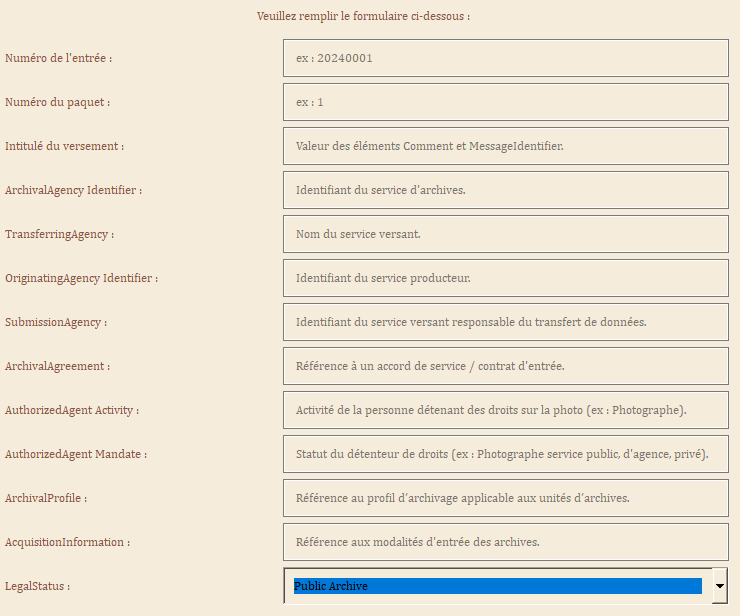
\includegraphics[width=\textwidth]{./img/orphee_formulaire_1.png}
\caption{Capture d'écran de la première partie du formulaire de l'application ORPhÉE.}
\end{figure}

Dans un second temps, le formulaire permet à l'utilisateur de choisir les métadonnées internes à extraire avec la librairie PyExiftool : chaque case cochée correspond à un champ de métadonnées que l’utilisateur souhaite extraire des fichiers pour l’ajouter au manifest. Nous évoquions dans le chapitre précédent la nécessité d'établir une priorité dans le choix des informations issues de plusieurs schémas de métadonnées : le guide utilisateur précise l'ordre établi pendant l'analyse des reportages de la Présidence de la République et adopté par l'application. Il est donc recommandé aux utilisateurs de procéder en amont à une analyse des métadonnées internes afin d'assurer une sélection des champs les plus pertinents. De plus, à l'instar de la première version de l'application, il est proposé de rattacher le paquet fabriqué à une unité archivistique déjà versée en cochant une case et en renseignant les informations nécessaires.

Le recours à ce formulaire permet notamment de revenir sur les informations renseignées, ce qui présente un avantage conséquent par rapport à la première version de l'application qui demandait les informations les unes après les autres et ne permettait pas de modifier une information déjà fournie.


\section{Pistes d'améliorations fonctionnelles}

\subsection*{Gestion des erreurs et validation du manifest}

L'application actuelle ne dispose pas encore d'un système de gestion des erreurs robuste. Par manque de temps, je n'ai pas pu intégrer un traitement interne des erreurs. Comme solution temporaire, j'ai répertorié les erreurs les plus fréquentes dans la documentation de l'application, en expliquant leur origine et en proposant des solutions possibles.

Par exemple, la présence de chemins trop longs ou de certains caractères spéciaux dans les noms de dossiers et de fichiers peut empêcher le bon fonctionnement de l'application, entraînant une erreur de balise vide. Les outils externes utilisés par l'application, tels que Siegfried et PyExiftool, ne reconnaissent pas ces chemins ou les excluent de leur traitement, ce qui peut provoquer deux types d'erreurs : une erreur lors de l'extraction des métadonnées, et une erreur lors de l'écriture du manifest. Lorsqu'un chemin contient un caractère spécial, il peut être mal interprété par l'application, qui ne parvient alors pas à retrouver le fichier dans l'arborescence. En conséquence, aucune métadonnée n'est récupérée, ce qui génère une erreur. Aussi, certains éléments associés aux fichiers dont le chemin pose problème ne sont pas créés, comme l'élément \xmlinline{<BaliseTemp>} qui devrait contenir l'empreinte calculée par Siegfried. Si cet élément n'est pas créé, l'application renvoie une erreur.

Une autre fonctionnalité que j'aurais souhaité pouvoir implémenter est la vérification de la validité du manifest en SEDA, avec une restitution des erreurs et des suggestions de solutions.

\subsection*{Optimisation des performances et scalabilité}

Une autre piste d'amélioration concerne l'optimisation du code : réviser l'ensemble des fonctions afin de déterminer s'il existe des opérations redondantes, ou des algorithmes complexes qui pourraient être simplifiés. Ces améliorations permettraient d'augmenter les performances de l'outil et de garantir qu'il puisse gérer une charge croissante de données sans perdre en efficacité.

La scalabilité désigne la capacité d'un système à s'adapter à une augmentation de la taille des données tout en maintenant des performances acceptables. Actuellement, la constitution d’un paquet de 20 Go prend entre 10 et 20 minutes, celle d’un paquet de 60 Go entre 20 et 30 minutes, et celle d’un paquet de 100 Go entre 40 minutes et 1 heure. Ce comportement linéaire du temps de traitement en fonction de la taille des données indique que le logiciel pourrait être optimisé pour améliorer la scalabilité.

\subsection*{Améliorations du formulaire}

Une autre amélioration possible serait l'ajout d'un fichier de configuration permettant de préremplir automatiquement certaines métadonnées dans le formulaire, en fonction du contexte d'utilisation. Par exemple, un service d'archives pourrait ainsi éviter de renseigner son identifiant à chaque utilisation de l'application.


\section{Maintenabilité de l'application}
L'application a été initialement conçue pour répondre à un besoin immédiat, ponctuel, et interne au Département de l'administration des données : l'automatisation de la reprise des reportages photographiques. L'objectif principal était donc de développer un outil qui reproduise les étapes définies lors de la modélisation du traitement des données. Ainsi, la pérennité de l'outil n'a pas été envisagée dès le départ. Une fois son efficacité avérée, la possibilité d'une utilisation par d'autres services d'archives a été envisagée. Cette nouvelle perspective nous a amené à nous interroger sur sa maintenabilité à l'issue du stage et du chantier de reprise. La notion de maintenabilité d'un logiciel renvoie à sa capacité à être facilement modifié, corrigé, ou amélioré au fil du temps. Elle dépend de la qualité du code, de sa modularité, de la clarté de la documentation, et de l'adoption de bonnes pratiques de développement.

Dans ce contexte, nous avons étudié les facteurs permettant de garantir la reprise de l'outil par d'autres utilisateurs. Chaque fonction a été documentée avec des \gls{docstrings}, avec l'ajout de commentaires spécifiques pour décrire les différentes étapes des fonctions les plus complexes. J'ai rédigé une documentation, mise en ligne sur GitHub. Cette documentation se divise en plusieurs parties: 

\begin{itemize}
	\item Un guide décrivant le format des données acceptées et les bonnes pratiques d'analyse et de nettoyage des données à réaliser en amont.
	\item Une présentation de l'interface utilisateur détaillant les différentes sections du formulaire et les messages de suivi des opérations.
	\item Une liste des erreurs les plus fréquentes, précisant leur origine et les moyens identifiés pour les solutionner.
	\item Une description du fonctionnement du code détaillant chacune des fonctions qui le constituent.
\end{itemize}

De plus, j'ai animé plusieurs réunions de présentation du code auprès des agents du DAD pour les tenir informés de son état d'avancement et de son fonctionnement global. À l'issue de l'une de ces réunions, nous avons évoqué les possibilités de réutilisation du code au delà de la reprise des reportages photographiques de la Présidence : il est par exemple envisageable de reprendre certaines fonctions pour la conception d'autres outils de fabrication de paquets d'archives, adaptés à des typologies différentes.

Pour garantir la pérennité du code et se prémunir contre les problèmes d'obsolescence ou de compatibilité, une gestion efficace des dépendances sera nécessaire par les services souhaitant utiliser l'application. Pour faciliter cette maintenance, la liste des librairies Python utilisées dans l'application est fournie sur mon Github, dans le fichier \enquote{requirements.txt}.
\\

Avoir travaillé sur le chantier de reprise des reportages photographiques aux Archives nationales au cours de mes deux stages de master m'a permis d'aborder le sujet sous deux perspectives à la fois différentes et complémentaires. Lors de mon travail de première année sur les reportages des services du Premier ministre, sans les connaissances et compétences numériques nécessaires pour traiter efficacement de grandes quantités de données, j'ai dû développer des expédients, des solutions semi-automatisées et chronophages. Cette approche m'a néanmoins donné l'opportunité de me concentrer pleinement sur les enjeux métier : modélisation des processus, nettoyage des données, analyse de l'existant, mappage des données et des métadonnées, etc. Le stage de deuxième année, en revanche, a été l'occasion de mettre à profit les compétences techniques acquises pour répondre non seulement à un besoin du service -- proposer une méthode de fabrication automatique de SIP pour les reportages photographiques de la Présidence de la République -- mais aussi à une curiosité personnelle née pendant mon premier stage : dans quelle mesure les technologies numériques peuvent-elles automatiser et accélérer les opérations réalisées manuellement l'année précédente ? J'ai ainsi pu créer un outil capable d'enchaîner les traitements modélisés l'année précédente, apportant une solution plus efficace. Bien sûr, l'application produite ne reprend pas exactement le travail de mon stage de 2023 : les données étant différentes, les solutions et les besoins ont également évolué : le mappage n'est pas identique, la volumétrie des données non plus, etc. Néanmoins, l'achèvement de ce projet m'a apporté la satisfaction d'avoir abouti à une solution complète et cohérente de bout en bout.